\begin{frame}{Three neuron motifs}

  % \begin{figure}
  %   \centering
  %   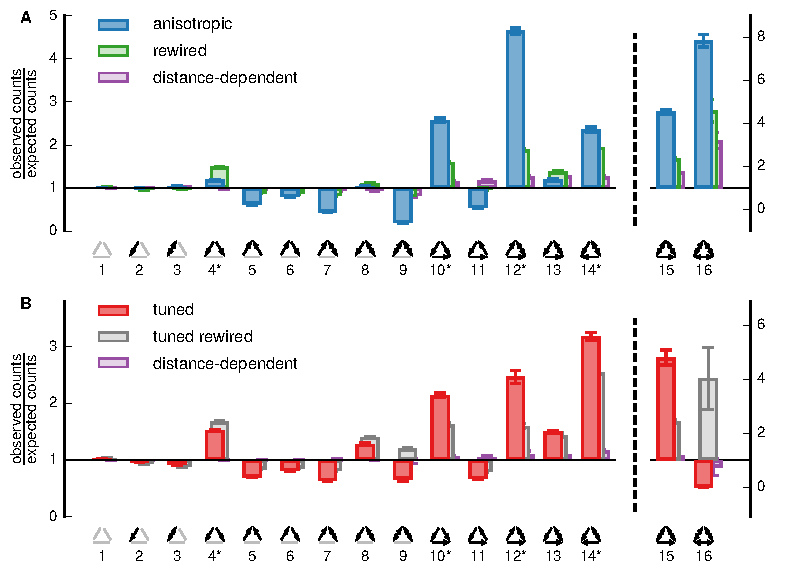
\includegraphics[width=\textwidth]{%
  %     figures/three_motifs_3x1.pdf} %
  % \end{figure}


  \begin{figure}
    \centering
    \includegraphics<1>[width=\textwidth]{%
      figures/fig4_3motif_aniso_bare.pdf}
    \includegraphics<2-3>[width=\textwidth]{%
      figures/fig4_3motif_aniso_bare_highlight.pdf}
    \includegraphics<4-5>[width=\textwidth]{%
      figures/fig4_3motif_aniso_rew.pdf}
    \includegraphics<6>[width=\textwidth]{%
      figures/figSI_3motif_aniso_relrew.pdf}
    \includegraphics<7>[width=\textwidth]{%
      figures/figSI_3motif_aniso_relrew_highlight.pdf}
    \includegraphics<8>[width=\textwidth]{%
      figures/fig4_3motif_aniso_rew.pdf}
    \includegraphics<9->[width=\textwidth]{%
      figures/fig4_3motif_aniso_full.pdf}

  \end{figure}

  \begin{figure}
    \centering
    \includegraphics<1-2>[width=0.8\textwidth]{%
      figures/Song2005_Fig4A.png}
    \includegraphics<3-4>[width=\textwidth]{%
      figures/fig4_3motif_tuned_bare.pdf}
    \includegraphics<5>[width=\textwidth]{%
      figures/fig4_3motif_tuned_rew.pdf}
    \includegraphics<8-9>[width=\textwidth]{%
      figures/fig4_3motif_tuned_rew.pdf}
    \includegraphics<10>[width=\textwidth]{%
      figures/fig4_3motif_tuned_full.pdf}
  \end{figure}
  

  


  % \source{Hoffmann \& Rotter, in prep.}
  
  
\end{frame}


